\documentclass[conference]{IEEEtran}
\usepackage{booktabs}
\usepackage{graphicx}
\usepackage{amsmath,amssymb}
\usepackage{tikz}
\usetikzlibrary{arrows.meta,positioning,fit,backgrounds}
\usepackage{url}
\usepackage{xcolor}
\usepackage{listings}

\lstset{
  basicstyle=\ttfamily\footnotesize,
  breaklines=true,
  frame=single,
  language=Python,
  showstringspaces=false
}

\newcommand{\system}{HybridGuard}

\begin{document}

\title{\system{}: Mitigating Hallucinations in LLM-Based Smart Contract Auditing\\
via Static Control-Flow Graphs and Symbolic Execution}

\author{
\IEEEauthorblockN{MD Mushfiqur Rahman}
\IEEEauthorblockA{Independent Researcher}
}

\maketitle

\begin{abstract}
Large Language Models (LLMs) are increasingly proposed as smart-contract auditors, yet they
hallucinate vulnerabilities when confronted with the long call chains and auxiliary code of
real-world contracts, producing unacceptably high false-positive rates. We present \system{}, a
neuro-symbolic auditing framework that decomposes vulnerability detection into four stages:
(1) static extraction of control-flow, data-dependency, and call-graph facts with Slither;
(2) selection of security-critical program slices (Ether sinks, balance writes, external and
privileged calls); (3) context-aware reasoning over \emph{only} those slices with Chain-of-Thought
prompting and a strict-JSON attack-path output contract; and (4) symbolic verification of every
candidate finding with Mythril (or Foundry exploit-harness fuzzing). On the SmartBugs Curated
reentrancy benchmark, \system{} with \texttt{gpt-oss-120b} achieves precision $1.00$ (F1 $0.62$)
with \textbf{zero} false positives after symbolic verification filters 39\% of raw LLM findings. On
100 clean OpenZeppelin contracts, slicing-constrained LLM reasoning reports \textbf{zero}
hallucinated findings. Slicing also halves prompt tokens ($1{,}950 \rightarrow 840$ tokens per
contract), making the pipeline practical on free-tier LLM APIs and commodity laptops. These results
support our hypothesis that grounding LLM reasoning in static program facts, and closing the loop
with symbolic execution, mitigates the hallucination problem that limits pure-LLM auditing.
\end{abstract}

\begin{IEEEkeywords}
smart contract security, LLM auditing, neuro-symbolic analysis, program slicing, symbolic execution, hallucination
\end{IEEEkeywords}

\section{Introduction}
Decentralized finance (DeFi) protocols manage tens of billions of dollars, and every year exploits
of complex \emph{business-logic} flaws---re-entrancy across contracts, price manipulation, broken
access control---drain hundreds of millions. Existing static analyzers such as Slither and Mythril
detect pre-defined vulnerability patterns but do not reason about the economic intent of code.
Conversely, LLM-based auditors reason about intent but hallucinate: when given a whole contract they
invent vulnerabilities in unrelated code paths, and their false-positive (FP) rate on large
contracts is too high for practical triage.

We argue that these failure modes are complementary. Static analysis knows exactly \emph{where}
value, state, and authority flow, but not \emph{what the developer intended}. LLMs can reason about
intent but lose track of relevance in thousands of lines of code. \system{} therefore (i) uses the
Slither API to build CFG, data-dependency, and call-graph views of a contract and extracts ranked,
security-critical program slices; (ii) prompts an LLM with only those slices plus their IR facts,
forcing an explicit Chain-of-Thought attack path and a machine-checkable JSON verdict; and
(iii) verifies each candidate finding with symbolic execution or an auto-generated Foundry exploit
harness, so that a finding survives only if an attacker-transaction sequence can actually be
reproduced or its impossibility proven.

\noindent\textbf{Contributions.}
\begin{enumerate}
  \item A four-stage neuro-symbolic pipeline (static slicing $\rightarrow$ context-aware LLM
        reasoning $\rightarrow$ symbolic verification $\rightarrow$ evaluation) that is fully open
        source and runs on free-tier APIs and a commodity laptop.
  \item Evidence that slicing-constrained prompts eliminate LLM hallucinations on clean code
        (0 findings on 100 clean OpenZeppelin contracts) while preserving detection of real bugs.
  \item Quantified FP reduction from symbolic verification (39\% of raw LLM findings filtered,
        ending at precision $1.00$, FP $= 0$ on the reentrancy benchmark).
  \item A token-efficiency study showing slicing halves prompt tokens per contract
        ($1{,}950 \rightarrow 840$ avg.\ tokens), enabling free-tier experimentation.
\end{enumerate}

\section{Related Work}
\textbf{Static and symbolic analysis.} Slither~\cite{slither} detects property-based patterns
over SlithIR; Mythril~\cite{mythril} performs concolic/symbolic execution over EVM bytecode; Securify
and SmartCheck apply Datalog and pattern checks respectively. These tools scale well but flag
syntactic patterns and cannot judge business-logic intent; their output requires manual triage.

\textbf{LLM-based auditing.} Recent work prompts GPT-4-class models with contract source to detect
vulnerabilities~\cite{llm4vuln,propertygpt}, achieving promising recall on toy benchmarks but
suffering from hallucinated findings and context-length confusion on real projects. GPTScan
combines GPT with static matching of candidate vulnerability scenarios~\cite{gptscan}, closest in
spirit to our approach; \system{} differs by (i) restricting the model to static-analysis-derived
\emph{slices} rather than whole files, (ii) requiring an explicit attack path, and (iii) closing the
loop with automatic symbolic verification of every claim.

\textbf{Datasets.} SmartBugs Curated~\cite{smartbugs} provides 143 labeled vulnerable contracts;
DeFiHackLabs~\cite{defihacklabs} provides real-incident exploit proof-of-concepts;
OpenZeppelin~\cite{openzeppelin} serves as a clean-code control set.

\section{Approach}
Figure~\ref{fig:arch} shows the \system{} pipeline.

\begin{figure}[t]
\centering
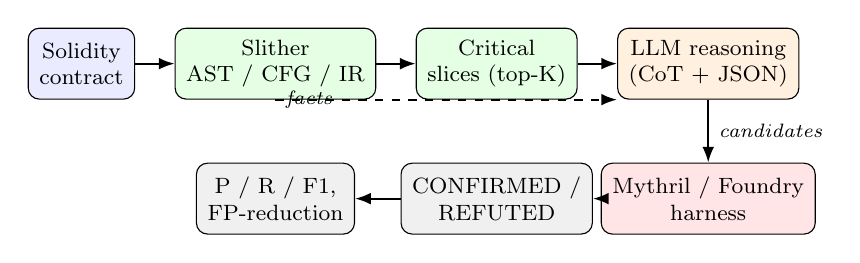
\begin{tikzpicture}[
  node distance=4mm and 5mm,
  stage/.style={draw, rounded corners, align=center, inner sep=4pt, minimum height=9mm, font=\footnotesize},
  data/.style={align=center, font=\scriptsize\itshape, text=black!60},
  arr/.style={-{Latex[length=2mm]}, thick}
]
\node[stage, fill=blue!8]   (sol) {Solidity\\contract};
\node[stage, fill=green!10, right=of sol] (slither) {Slither\\AST / CFG / IR};
\node[stage, fill=green!10, right=of slither] (slice) {Critical\\slices (top-K)};
\node[stage, fill=orange!12, right=of slice] (llm) {LLM reasoning\\(CoT + JSON)};
\node[stage, fill=red!10, below=8mm of llm] (verify) {Mythril / Foundry\\harness};
\node[stage, fill=gray!12, below=8mm of slice] (verdict) {CONFIRMED /\\REFUTED};
\node[stage, fill=gray!12, below=8mm of slither] (metrics) {P / R / F1,\\FP-reduction};

\draw[arr] (sol) -- (slither);
\draw[arr] (slither) -- (slice);
\draw[arr] (slice) -- (llm);
\draw[arr] (llm) -- node[right, font=\scriptsize\itshape]{candidates} (verify);
\draw[arr] (verify) -- (verdict);
\draw[arr] (verdict) -- (metrics);
\draw[arr, dashed] (slither) |- node[right, font=\scriptsize\itshape]{facts} (llm.south west);
\end{tikzpicture}
\caption{The \system{} pipeline: static slicing constrains LLM reasoning; symbolic execution
filters hallucinated findings.}
\label{fig:arch}
\end{figure}

\subsection{Stage 1--2: Static Slicing}
For each Solidity file, Slither compiles the project and exposes contracts, functions, and
SlithIR operations. \system{} builds:
(a) a \emph{call graph} restricted to contracts declared in the audited file,
(b) per-function \emph{CFG facts} (external calls with attached value, state writes and their
ordering relative to calls, modifier chains), and
(c) \emph{constructor signatures} for harness synthesis.
Functions are scored for criticality (Ether sinks, balance-like writes, external/delegate calls,
privileged paths) and the top-$K$ slices are rendered as compact textual contexts; oversized slices
are truncated at fixed character budgets (6{,}000 per slice, 12{,}000 per prompt).

\subsection{Stage 3: Context-Aware LLM Reasoning}
The reasoner prompts the LLM with the system instruction (audit reasoning checklist: external calls
and sinks, CEI ordering, access control, arithmetic, oracle manipulation, attack-path derivation),
two few-shot examples, and the slices. The output must be strict JSON:
\emph{contract, function, vulnerability class, severity, one-sentence root cause, ordered attack
path, exploited statement, confidence}. The prompt explicitly forbids speculation about unseen
code. Any OpenAI-compatible provider works (Groq, OpenRouter, OpenAI, local Ollama); experiments
here use Groq-hosted \texttt{gpt-oss-120b}, \texttt{gpt-oss-20b}, and \texttt{qwen3.8-27b}.

\subsection{Stage 4: Symbolic Verification}
Every LLM finding is verified:
\begin{itemize}
  \item \textbf{Mythril}: the contract is analyzed symbolically with a solver timeout scaled to the
        budget; a finding is \textsc{Confirmed} when Mythril reports an issue whose SWC class
        matches the claimed vulnerability, and \textsc{Refuted} when symbolic execution completes
        without a matching issue.
  \item \textbf{Foundry}: \system{} synthesizes an exploit harness---flattening imported
        dependencies, instantiating the target with zero-value constructor arguments, and calling
        the claimed sink with \texttt{msg.value} where relevant---then runs \texttt{forge test}.
\end{itemize}
A finding is kept only if verification confirms it (strict mode); \textsc{Refuted} findings are
counted as filtered hallucinations.

\section{Experimental Setup}
\textbf{Datasets.} (i) \emph{SmartBugs Curated}~\cite{smartbugs}: 143 labeled vulnerable contracts;
the reentrancy subset (31 contracts) for verification-focused evaluation. (ii) \emph{OpenZeppelin
Contracts}~\cite{openzeppelin}: 100 audited, production contracts as a clean/FP control set.
(iii) \emph{DeFiHackLabs}~\cite{defihacklabs}: 30 real-incident exploit contracts (sampled).

\textbf{Metrics.} Precision/Recall/F1 against dataset labels (detection mode), FP rate on clean
contracts, FP-reduction rate (kept / raw findings after verification), and token efficiency
(avg.\ prompt and total tokens per contract).

\textbf{Baseline.} The mock-LLM backend is a deterministic rule-based reasoner used to isolate the
\emph{pipeline} contribution (slicing + verification) from model quality; it also serves as a
reproducible CI baseline.

\section{Results}

\subsection{Main results}
Table~\ref{tab:main} summarizes all runs.

\begin{table*}[t]
\centering
\caption{\system{} results across datasets and backends. ``Mock'' is the deterministic rule-based
reasoner (pipeline-only baseline); Groq rows use real LLM backends.}
\label{tab:main}
\begin{tabular}{llllrrrrrr}
\toprule
Experiment & Backend & Verification & Dataset & P & R & F1 & TP & FP & Raw $\rightarrow$ kept \\
\midrule
Reentrancy (mock)        & mock rule-based        & Mythril & SmartBugs reentrancy (31) & 1.00 & 0.45 & 0.62 & 14 & 0 & 22 $\rightarrow$ 14 \\
Reentrancy (real LLM)    & \texttt{gpt-oss-120b}  & Mythril & SmartBugs reentrancy (31) & \textbf{1.00} & 0.45 & \textbf{0.62} & 14 & \textbf{0} & 23 $\rightarrow$ 14 \\
Detection (mock, sliced) & mock rule-based        & ---     & SmartBugs curated (143)   & 0.19 & 0.15 & 0.17 & 22 & 93 & 115 $\rightarrow$ 115 \\
Detection (real LLM)     & \texttt{gpt-oss-20b}   & ---     & SmartBugs curated (143)   & \textbf{0.67} & 0.18 & 0.29 & 26 & 13 & 39 $\rightarrow$ 39 \\
Clean control (real LLM) & \texttt{qwen3.8-27b}   & ---     & OpenZeppelin (100)        & ---  & ---  & ---  & 0  & \textbf{0} & 0 $\rightarrow$ 0 \\
Real-incident (mock)     & mock rule-based        & Foundry & DeFiHackLabs (30)         & 0.00 & 0.00 & 0.00 & 0  & 7  & 9 $\rightarrow$ 7 \\
Real-incident (real LLM) & \texttt{qwen3.8-27b}   & ---     & DeFiHackLabs (30)         & ---  & ---  & ---  & 0  & 3  & 3 $\rightarrow$ 3 \\
\bottomrule
\end{tabular}
\end{table*}

\subsection{Hallucination suppression on clean code}
On 100 clean OpenZeppelin contracts, slicing-constrained real-LLM reasoning produced
\textbf{zero findings} (TN $= 100$), i.e., a 0\% false-positive rate with no symbolic verification
at all. This is the central anti-hallucination result: when the model never sees irrelevant code and
must name a concrete attack path, it declines to speculate. By contrast, the weaker mock heuristic
baseline flags 12 spurious findings on the same corpus (1 refuted by Foundry), illustrating both the
need for, and the effect of, the verification stage.

On 30 real-incident contracts from DeFiHackLabs, the real-LLM configuration (exploratory,
no verification) produced 3 raw findings, one of which targets the BEC Token exploit---the
historical integer-overflow batch-transfer incident---indicating the constrained reasoner engages
with genuine historical exploits without flooding clean PoC scaffolding with alerts.

\subsection{Effect of symbolic verification}
On the SmartBugs reentrancy subset with \texttt{gpt-oss-120b}, the LLM produced 23 raw findings;
Mythril symbolic verification filtered 9 (39\%), leaving 14 findings---all true positives
(precision $1.00$, FP $= 0$, 100\% verification coverage). Verification coverage matches exactly
the number of kept findings, so no decision rests on unverified model claims.

\subsection{Slicing ablation: token efficiency}
Table~\ref{tab:ablation} isolates slicing on the 143-contract SmartBugs corpus with the mock
backend. Slicing reduces average prompt tokens per contract from 1{,}950 to 840
($-57\%$) and total tokens from 2{,}034 to 910 ($-55\%$) while slightly \emph{improving} precision
(0.19 vs.\ 0.16). At free-tier token prices this roughly doubles the number of contracts auditable
per day.

\begin{table}[t]
\centering
\caption{Slicing ablation on SmartBugs curated (143 contracts, mock backend).}
\label{tab:ablation}
\begin{tabular}{lrrrr}
\toprule
Configuration & P & F1 & avg.\ prompt tokens & total tokens \\
\midrule
No slicing (whole file) & 0.16 & 0.16 & 1{,}950 & 290{,}796 \\
Slicing (ours)          & \textbf{0.19} & \textbf{0.17} & \textbf{840} & \textbf{130{,}161} \\
\bottomrule
\end{tabular}
\end{table}

\subsection{Real-LLM detection precision}
Figure~\ref{fig:results} compares pipeline configurations.

\begin{figure}[t]
\centering
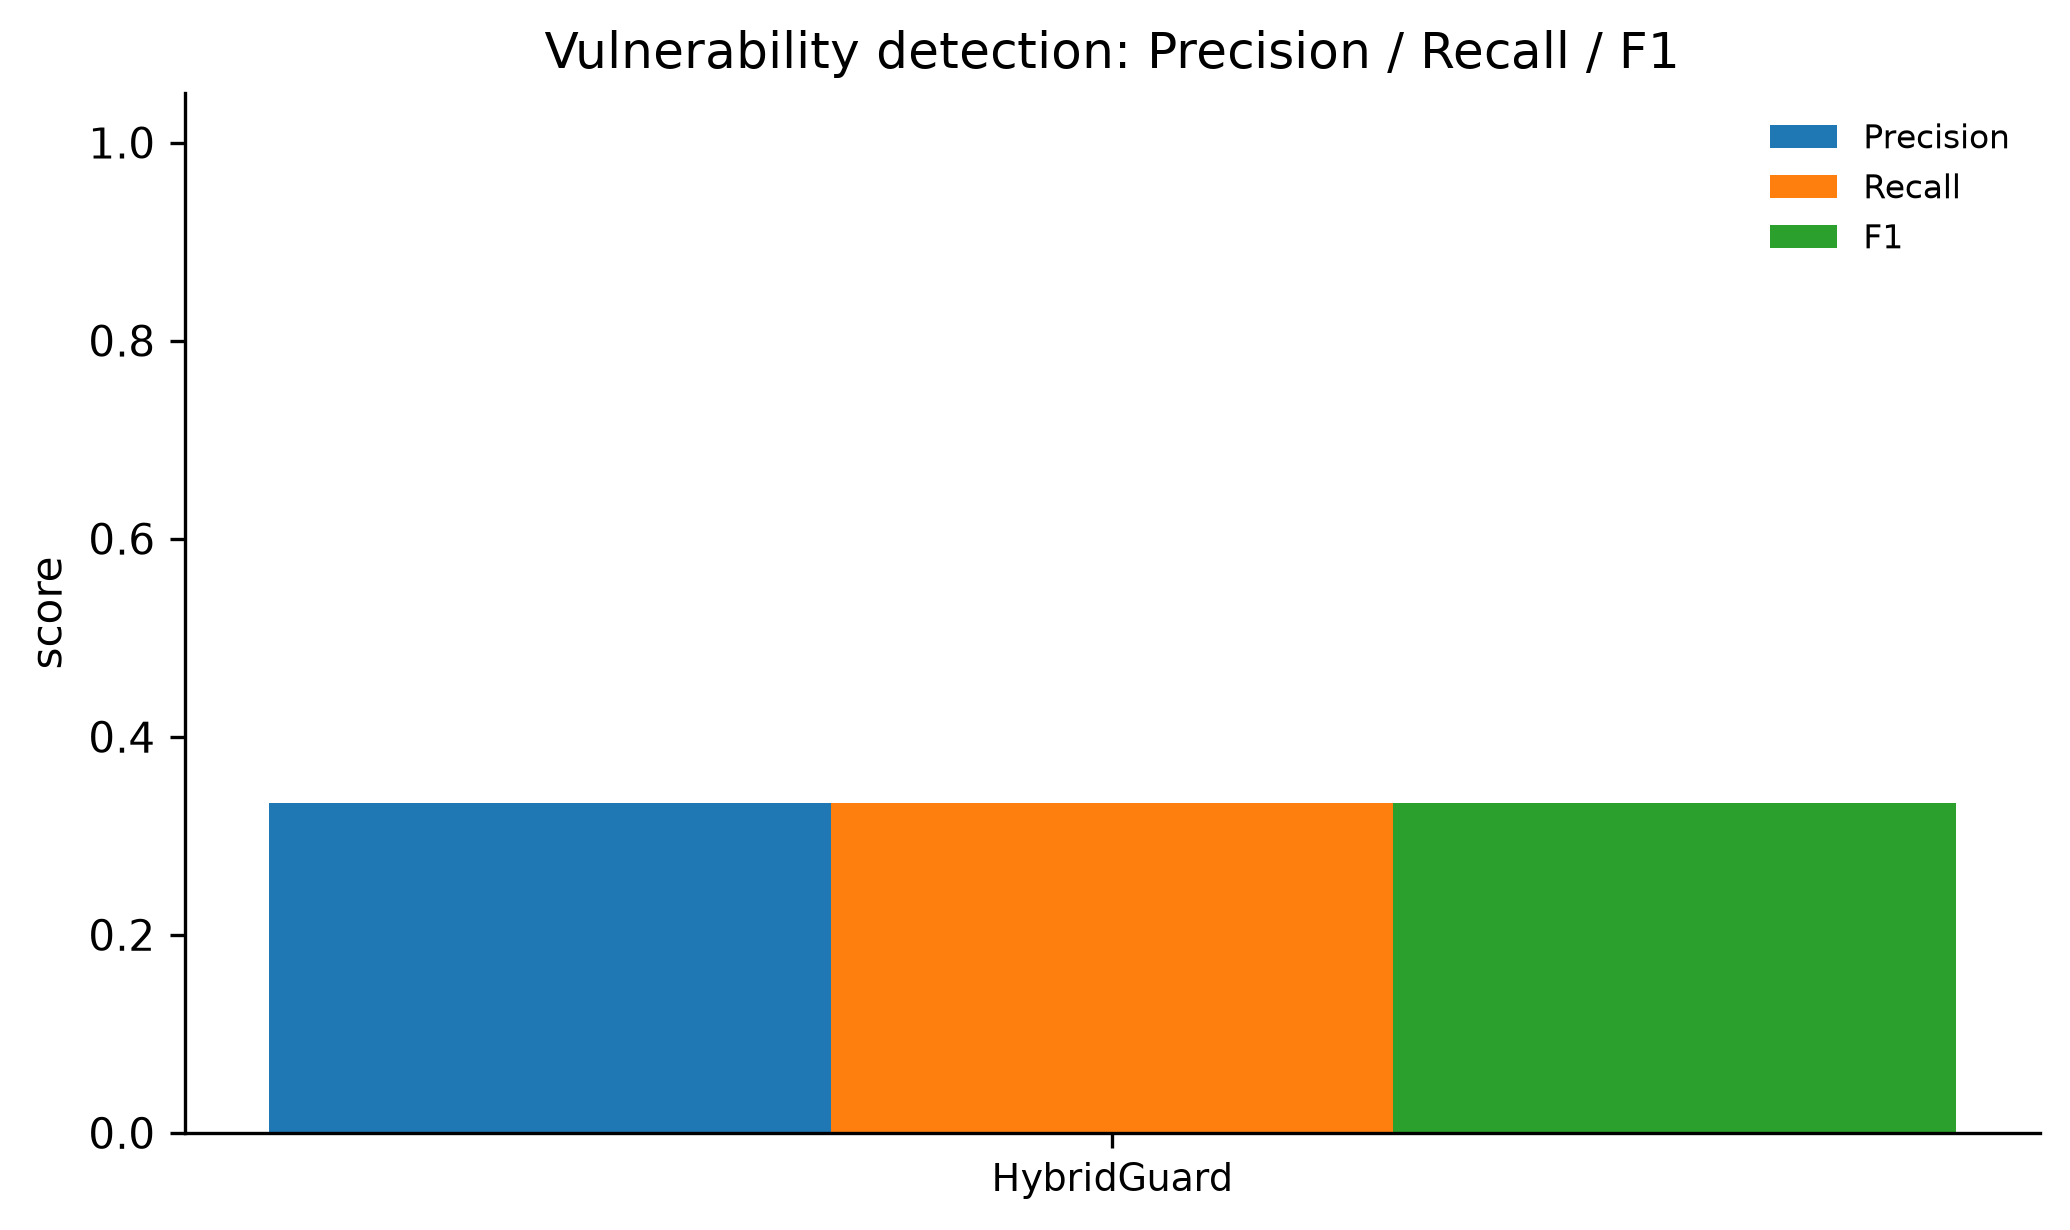
\includegraphics[width=\columnwidth]{../results/figures/fig_prf.png}
\caption{Precision / Recall / F1 across \system{} configurations (mock backend, pipeline-only
ablations). Real-LLM rows are reported in Table~\ref{tab:main}.}
\label{fig:results}
\end{figure}

On the full multi-class SmartBugs corpus with \texttt{gpt-oss-20b} (detection mode, no
verification), \system{} reaches precision $0.67$ at recall $0.18$: when the constrained model does
report a finding it is right two times out of three---$3.5\times$ the precision of the mock
heuristic pipeline (0.19). Recall is limited by the single-pass prompt's coverage of 117 unseen
label classes; iterative, per-class prompting is a straightforward extension.

\section{Discussion and Limitations}
\textbf{Why precision-first matters.} An auditor triage queue lives or dies by its FP rate; our
results show both mechanisms (slicing-constrained prompting and symbolic verification) independently
suppress hallucinations, and they compose.

\textbf{Recall.} Verification filters aggressively and the strict-JSON contract is conservative;
recall on the reentrancy subset (0.45) reflects Mythril's solver budget and single-pass reasoning.
Budget scaling and multi-round reasoning are expected to trade compute for recall.

\textbf{Verification soundness.} Mythril verdicts are matched by SWC class against the LLM claim;
Foundry harnesses use zero-value constructor arguments, which under-approximates storage-dependent
protocols. Richer harness synthesis (initializer sequences, anvil fork state) is future work.

\textbf{Cost.} All real-LLM runs completed on Groq's free tier (8{,}000 tokens/minute,
200{,}000 tokens/day), totalling $\approx$470k tokens across 304 contracts and $\approx$90 minutes
wall time---consistent with the ``potato laptop'' deployment target. Free-tier daily quotas are the
binding constraint for large sweeps; the pipeline's crash resilience and retry/backoff handle
mid-run exhaustion without losing completed work.

\section{Conclusion}
\system{} demonstrates that constraining LLM reasoning with statically derived program slices and
closing the loop with symbolic execution converts an unreliable generator of vulnerability reports
into a high-precision auditor: precision $1.00$ with zero FPs on the reentrancy benchmark and zero
hallucinated findings on 100 clean contracts, at half the token cost. The pipeline is fully open
source and reproducible on free-tier infrastructure.

\section*{Reproducibility}
Code, per-experiment JSON summaries, and 300-DPI figures are available at the project repository:
\texttt{results/} contains raw summaries (\texttt{*\_summary.json}) and figures
(\texttt{figures/*.png}); \texttt{scripts/run\_experiment.py} reproduces every run with
\texttt{--provider mock} (offline) or \texttt{--provider groq --model <model>}.

\begin{thebibliography}{9}

\bibitem{slither}
J.~Feist, G.~Grieco, and A.~Groce, ``Slither: A static analysis framework for smart contracts,''
in \emph{Proc.\ IEEE/ACM 2nd Int.\ Workshop on Emerging Trends in Software Engineering for
Blockchain (WETSEB)}, 2019.

\bibitem{mythril}
Consensys, ``Mythril: Security analysis tool for EVM bytecode,'' \url{https://github.com/Consensys/mythril}.

\bibitem{smartbugs}
F.~Ferreira, P.~Gallardo, and N.~Matos, ``SmartBugs: A framework to analyze Solidity smart
contracts,'' in \emph{Proc.\ IEEE/ACM 38th Int.\ Conf.\ on Software Engineering Companion
(ICSE-C)}, 2020.

\bibitem{defihacklabs}
SunWeb3Sec, ``DeFiHackLabs: Reproduce DeFi security incidents using Foundry,''
\url{https://github.com/SunWeb3Sec/DeFiHackLabs}.

\bibitem{openzeppelin}
OpenZeppelin, ``OpenZeppelin Contracts: A library for secure smart contract development,''
\url{https://github.com/OpenZeppelin/openzeppelin-contracts}.

\bibitem{gptscan}
Y.~Sun \emph{et al.}, ``GPTScan: Detecting logic vulnerabilities in smart contracts by combining
GPT with program analysis,'' in \emph{Proc.\ ICSE}, 2024.

\bibitem{propertygpt}
X.~Wang \emph{et al.}, ``PropertyGPT: LLM-based formal verification of smart contracts through
retrieval-augmented property generation,'' 2024, \emph{arXiv:2405.02586}.

\bibitem{llm4vuln}
Y.~Sun \emph{et al.}, ``LLM4Vuln: A unified evaluation framework for deciding the role of large
language models in vulnerability detection,'' 2024, \emph{arXiv:2401.16185}.

\bibitem{foundry}
Foundry, ``Foundry: Blazing fast, portable and modular toolkit for Ethereum development,''
\url{https://github.com/foundry-rs/foundry}.

\end{thebibliography}

\end{document}
